%!TEX root = main.tex
\section{Towards Dataset Understanding\label{sec:understanding}}
\subsection{Challenges}
\begin{itemize}
\item Problem of cold-start recommendation (as discussed earlier use may not always know what to query for)
\item related works have focussed on making specification easier , but not really trying to understnad user intent or what might the user want to see.
\item Within a dataset, structure and provenance is essential to help users navigate and provide users with sense of coverage and completion. This is an important but underexplored area. (viz-sum, Sarvghad et al 2017)
\item provenance of schema and attribute understanding (coverage, etc) 
\end{itemize}

\subsection{Examples}
\begin{itemize}
	\item understanding distributions (distribution awareness)
	\item providing overview recommendations (representative trends and outliers)
\end{itemize}

\subsection{\sbd: Navigating Through Data Slices with Hierarchical Summary of Visualizations}

\begin{figure}[h!]
\label{fig:modalities}
\centering
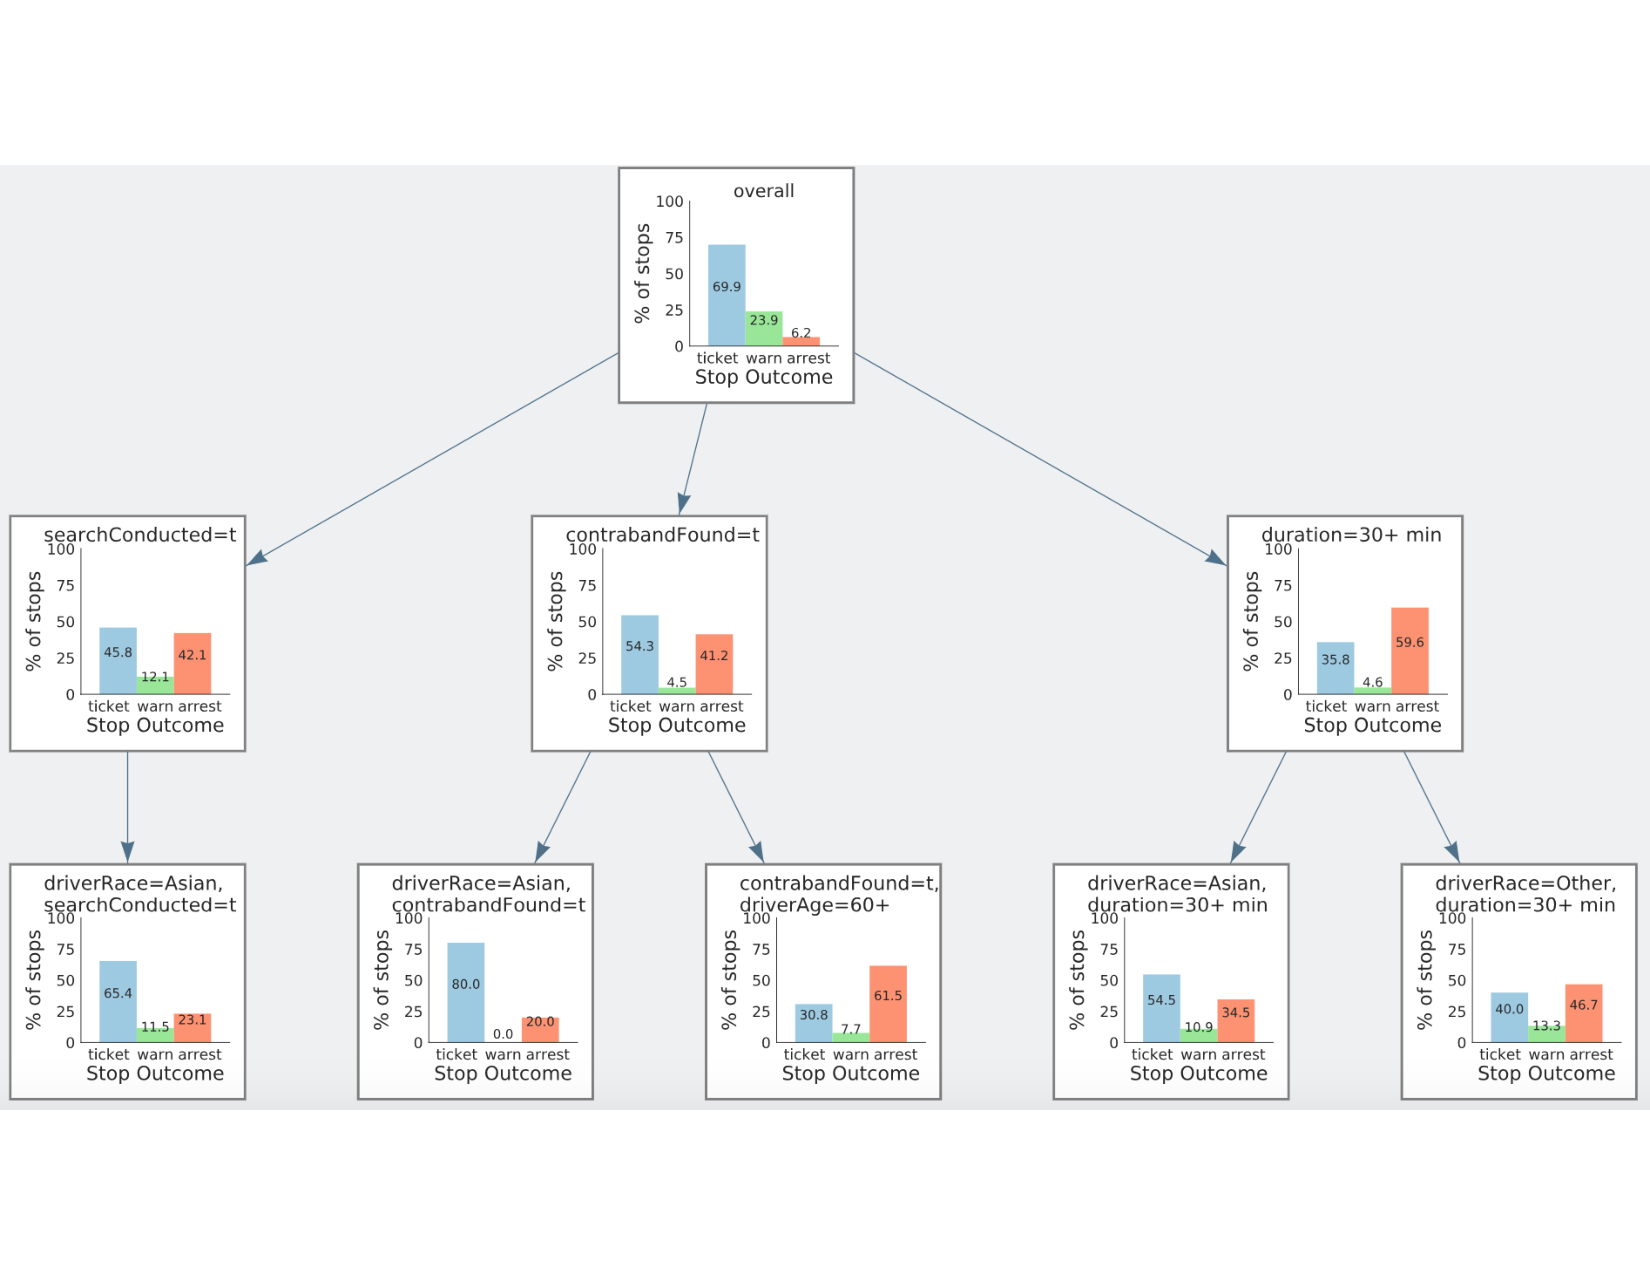
\includegraphics[width=0.7\linewidth]{figures/storyboard.pdf}
\caption{Example dashboard with generated from the Police Stop Dataset \cite{police}, which contains records of police stops that resulted in a warning, ticket, or an arrest.The attributes in the dataset include driver gender, age, race, and the stop time of day, whether a search was conducted, and whether contraband was found. We generate a dashboard of visualizations with bar charts with x-axis as the stop outcome (whether the police stop resulted in a ticket, warning, or arrest/summons) and y-axis as the percentage of police stops that led to this outcome.}
\end{figure}

Data is agnostic to the user, intention ---, by building tools---, Section \ref{sec:precise} to \ref{sec:vague} have focussed on extracting what user want from data. bridging together what user want from data, what data has to offer, supporting interactive discourse between the two. 
 Either using one-size-fits-all statistics, templates, heuristics as a solution or problem only applicable to a subset of analytic tasks\cite{Vartak2015,Vartak2017}. 
